\documentclass[a4paper,twocolumn]{article}

\usepackage{url}
\usepackage{graphicx}
\usepackage{emap}

% \usepackage{xcoffins}

\begin{document}

\headerauthor{Val\'eria de Paiva,Alexandre Rademaker,Gerard de Melo}
\headertitle{OpenWordNet-PT: an open Brazilian Wordnet for reasoning}
\headeryear{2012}
\cover

\title{OpenWordNet-PT: An Open Brazilian Wordnet for
  Reasoning~\thanks{We would like to thank Francis Bond for help in
    getting OpenWordNet-PT online and for general discussions. We also
    thank Adam Pease for introducing us and helping to start this
    project.}}

\author{Valeria de Paiva~\thanks{School of Computer Science, University of Birmingham, England} 
  \and Alexandre Rademaker~\thanks{Escola de Matem\'{a}tica Aplicada, FGV, Brazil} 
  \and Gerard de Melo~\thanks{ICSI, Berkeley, USA}}

\maketitle

\begin{abstract}
  Brazilian Portuguese needs a Wordnet that is open access,
  downloadable and changeable, so that it can be improved by the
  community interested in using it for knowledge representation and
  automated deduction. This kind of resource is also very valuable to
  linguists and computer scientists interested in extracting and
  representing knowledge obtained from texts. We discuss briefly the
  reasons for a Brazilian Portuguese Wordnet and the process we used
  to get a preliminary version of such a resource.  Then we discuss
  possible steps to improving our preliminary version.

  \textbf{Keywords}: Wordnet, Portuguese, lexical resources, SUMO
  Ontology.
\end{abstract}


\section{Motivation}

WordNet~\cite{wordnet} is an extremely valuable resource for research
in Computational Linguistics and Natural Language Processing in
general.  WordNet has been used for a number of different purposes in
information systems, including word sense disambiguation, information
retrieval, automatic text classification, automatic text
summarization, and dozens of other knowledge intensive projects.

We started a project at Funda\c{c}\~ao Getulio Vargas (FGV) in Brazil,
whose goal, in the long run, is to use formal logical tools to reason
about knowledge obtained from texts in Portuguese.
Originally we had expected to be able to use some existing Brazilian
Wordnet, out of the box, but it turns out that these are not available
in the form that we need it.  There are some attempts.

There is the project WordNet.PT (Portuguese WordNet) from the ``Centro
de Linguistica da Universidade de Lisboa'' headed by Prof. Palmira
Marrafa.  But this is available online only, no download available
and, as far as we can see on their webpages, little development has
happened recently to this project. The WordNet.PT version available
online has about 19000 lexical expressions, from different semantic
fields.  The fragment made available online includes expressions from
subdomains such as art, clothing, geography, health, institutions,
living entities and transportation, but no description of other
domains and/or future releases of the database are discussed. The
group has also a newer version of WordNet.PT called
$\texttt{WordNet.PT}_{\texttt{global}}$~\cite{mam:2011:DIALECTS} which
pays attention to different varieties of Portuguese, like African
variations of the language. But while this is very interesting for
linguistic comparative research and useful for online queries
(\url{http://www.clul.ul.pt/wnglobal/}), this smaller version of
WordNet.PT is not available for download and hence cannot  be the target of modifications and
improvements.

There is also the MultiWordNet project and its Portuguese version
MWN.PT, developed by Ant\^onio Branco and colleagues at the
NLX-Natural Language and Speech Group, of the University of Lisbon,
Department of Informatics. According to their
description~(\url{http://mwnpt.di.fc.ul.pt/}), MWN.PT, the
MultiWordnet of Portuguese (version 1), spans over 17,200 manually
validated concepts/synsets, linked under the semantic relations of
hyponymy and hypernymy. These concepts are made of over 21,000 word
senses/word forms and 16,000 lemmas from both European and American
variants of Portuguese. It includes the sub-ontologies under the
concepts of Person, Organization, Event, Location, and Artworks, which
are covered by the top ontology made of the Portuguese equivalents to
all concepts in the 4 top layers of the English Princeton WordNet and
to the 98 Base Concepts suggested by the Global Wordnet Association,
and the 164 Core Base Concepts indicated by the EuroWordNet
project. But again this wordnet is available online only and with a
restrictive license that requires payment.

Finally, there is a first version of a Brazilian Portuguese version of
Wordnet developed by Bento Dias da Silva and
collaborators~\cite{bento,carolina}. But this also cannot be
downloaded, is not available online and is not being maintained on an
open access basis, which is one of the strongest points of Princeton
WordNet.

Open access availability is one of the main reasons we would like to
create a new Portuguese Wordnet, which we are calling OpenWordNet-PT
(or OpenWN-PT for short). This is because we believe that resources
like Wikipedia and WordNet need to be open and modifiable by others in
order to improve over time.

With a similar philosophy of open access to ours, there is also the
work of Hugo Oliveira and Paulo Gomes on Onto.PT (\cite{ontoPT}),
another lexical ontology for the Portuguese language, structured
similarly to Princeton's WordNet, in the process of development at the
University of Coimbra, Portugal. Unlike our own OpenWordNet-PT,
Onto.PT is not connected to the synsets in the  Princeton WordNet. 
Due to this, existing Princeton WordNet-focused resources like
inter-lingual links in EuroWordNet, mappings to the SUMO ontology and
DBpedia/YAGO cannot be used in conjunction with this resource.

\section{OpenWordNet-PT}

OpenWordNet-PT is being created by drawing on a two-tiered methodology
so as to offer high precision for the more salient and frequent words
of the language, but also high recall in order to cover a wide range
of words in the long tail. We thus combine manual base concept
annotation with statistical cross-lingual projection techniques.

\subsection{Cross-Lingual Projection}

As a starting point, we applied the UWN/MENTA methodology
\cite{deMelo2009,de2010menta}, developed by one of the authors of this
paper in conjunction with Gerhard Weikum, to the Portuguese language.

In a first step, the information in the English Princeton WordNet is
projected to Portuguese by using translation dictionaries to map the
English members of a synset to possible Portuguese translation
candidates. In order to disambiguate and choose the correct
translations, feature vectors for possible translations are created by
computing graph-based statistics in the graph of words, translations,
and synsets. Additional monolingual wordnets and parallel corpora are
used to enrich this graph. Finally, statistical learning techniques
are then used to iteratively refine this information and build an
output graph connecting Portuguese words to synsets.

In a second step, Wikipedia pages are linked to relevant WordNet
synsets by learning from similar graph-based features as well as gloss
similarity scores.  Such mappings allow us to attach the article
titles of the Portuguese Wikipedia with WordNet synsets, thus further
increasing the coverage.


\subsection{Base Concept Annotation}

Using cross-lingual projection, we obtain a resource with good
coverage.  In order to have high precision for the most important
concepts of a language, we rely on human annotators.

In particular, we decided to rely on a set of Base Concepts.  The
Global WordNet Association aims at the development of wordnets for all
languages of the world and to extend the existing wordnets to full
coverage and many parts-of-speech. In 2006, the association launched a
project to start building a completely free worldwide wordnet
``grid''. This grid would be built around a shared set of concepts,
which would be expressed in terms of the original Wordnet synsets and
SUMO~\cite{niles2001towards} terms.

The vision of a global grid of wordnets in many languages that draw on
a common set of concepts is very appealing, as it enables many
cross-lingual applications.  The suggestion of the Global WordNet
Association is to build a first version of the grid around the set of
4689 ``Common Base Concepts'' and to make the grid free, following the
example of the Princeton WordNet. The Base Concepts are supposed to be
the most important concepts in the various wordnets of different
languages. The importance of the concepts was measured in terms of two
main criteria: (1) A high position in the semantic hierarchy; (2)
Having many relationships to other concepts.  The procedure described
as the EuroWordNet ``expand approach'' seemed sensible: First
translate the synsets in the Princeton WordNet to Portuguese, then
take over the relations from Princeton and revise, adding the
Portuguese terms that satisfy different relations. Then we hope to
revise thoroughly to guarantee the consistency of the taxonomy and to
make sure that all lexical items with a heavy use in Portuguese were
described. This process is under development at the moment. Currently,
Portuguese annotators are revising the base concepts by manually
choosing appropriate Portuguese words and by manually writing
appropriate Portuguese gloss descriptions.

\subsection{Project Status}

OpenWordNet-PT is freely available as an open-source
project\footnote{\url{https://github.com/arademaker/wordnet-br/}}.
The data is also available for online
browsing\footnote{\url{http://casta-net.jp/~kuribayashi/cgi-bin/wn-multi.cgi}}
via the online interface developed by Francis Bond
\cite{survey-wordnet}.  This interface, depicted in Fig. \ref{fig:ui},
is particularly insightful, as it displays Portuguese entries in
conjunction with entries in several other languages given by other
open-source wordnet projects.

\begin{figure}[htbp]
  \centering
  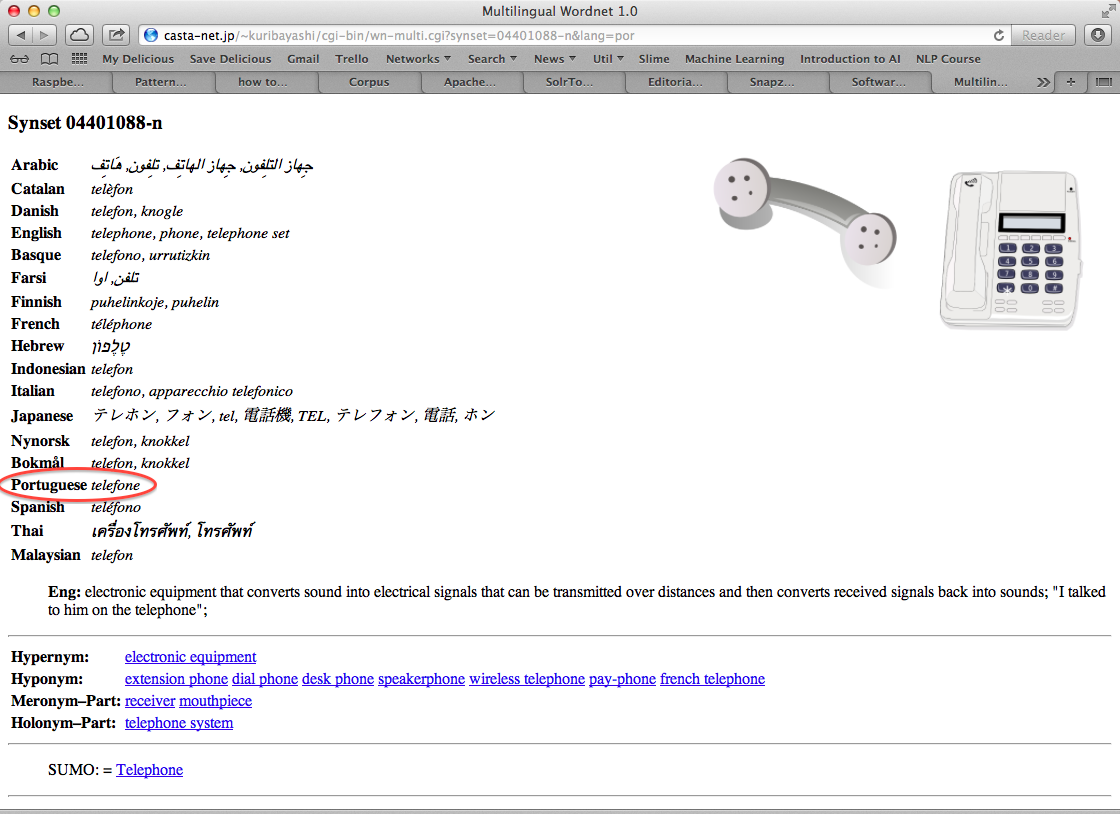
\includegraphics[width=.45\textwidth]{francis.png}
  \caption{Francis Bond's Open Multilingual Wordnet website}
  \label{fig:ui}
\end{figure}

In total, our resource has
62,034 sense-word pairs, and 45,421 unique words. These include 2,498
manually entered sense-word pairs as well as an additional 1,299
manually written Portuguese synset glosses.  Additional statistics
regarding the lexical coverage are provided in the appendix.

The raw coverage seems reasonable in number of terms in the ontology,
but we need to make sure that the quality of the items is comparable
and in particular that the level of detail is approximately the right
one for our intended application.

\section{Perspectives}

\subsection{OpenWordNet-PT and SUMO}

We started from an informal project discussing how logic and automated
reasoning could have a bigger impact, if coupled with natural language
processing. We also wanted to make sure that we could obtain some
(ideally most) of the advances already made for English text
understanding to Portuguese text understanding and reasoning.

Building on previously developed technology, like the Xerox PARC XLE
(Xerox Language Engine) system and trying to adapt that system to
Brazilian Portuguese seemed a good idea.  However, the AI and logic
components of the system come at the end of a long pipeline of modules
which require expertise on processing of natural language. In
particular we felt that a Brazilian Portuguese version of WordNet that
could be freely distributed to others was an essential part of it.


Wordnet is an important component of the XLE Unified Lexicon
(UL~\cite{crouch2005}), as the logical formulae created by the
Abstract Knowledge Representation (AKR) component of the system are
given meaning, in terms of Wordnet synsets. A previous version of the
system used, instead of the Unified Lexicon, the proprietary
Cyc~\cite{cyc} concepts as semantics. As discussed in \cite{til2} the
sparseness of Cyc concepts was the main reason to move away from Cyc
onto a version of the Bridge system based on the unified lexicon and WordNet.

Having a Brazilian version of WordNet and a mapping from Portuguese
words to that would allow us to use a knowledge representation system
very similar to the AKR (Abstract Knowledge Representation) used in
the PARC Bridge system. Having our version of the Portuguese WordNet based
on basic concepts we hope to leverage the huge manual construction
effort which constitutes the mapping from WordNet to
SUMO~\cite{sumo-mapping}. 

Through a
partnership with Adam Pease, (the technical editor of SUMO), 
%introduced the three of us, 
we additionally intend to use the SUMO hierarchy to
check the consistency between the Portuguese version of WordNet and
the English one.

\subsection{Intended Application}

The main application we envisage for our work in OpenWordNet-PT is
related to the entries in the Brazilian Dictionary of Historical
Biographies (in Portuguese DHBB), one of the main knowledge resources
implemented as a result of the archival efforts of the Funda\c{c}\~ao
Getulio Vargas.  The DHBB consists of 7,553 dictionary entries, out of
which 6,584 are biographies of important politicians in Brazil's
recent history. There are also 969 topical entries, concerning
institutions, events and descriptions relating to the history and
economy of Brazil after 1930. The dictionary is available 
online, but since the project was started in the 1970s the information
is not properly linked, which makes querying its data somewhat
unwieldy.

We intend to process all of the DHBB entries and we plan to extract from
them the main SUMO concepts referenced. Using these main SUMO concepts
we want to bootstrap a fledgeling Ontology of Historical Biographies,
already started and documented in the Development section of
SUMO. From the analysis of the SUMO concepts uncovered in the
biographical entries, we want to discover new relationships between
the historical characters described in the DHBB.

Here are some examples of the kinds of questions that this association
of text of biography entry with collections of SUMO concepts will
allow us to answer: 
% \begin{itemize}
% \item 
(1) Amongst Brazilian first rank politicians how many are from S\~ao
Paulo?
% \item 
(2) Has the proportion of Paulistas increased of decreased since the
1930s? Since 1965 when Brasilia became the Capital of Brazil has the
proportion changed?
% \item 
(3) What are the important Brazilian political families, corresponding
to the Kennedys, the Bushs, etc?
% \item 
(4) What are the prevalent occupations among Brazilian historical
figures? Are they mostly lawyers by training?
% \end{itemize}

\section{Conclusion} 

OpenWordNet-PT combines high recall with high precision for the more
salient words in the language. The work in this project is only
starting, but we have many plans to measure and increase the quality
of the Portuguese lexical resource, as well as many plans to use the
resource in its current form. The data is freely available for
download as well as for online browsing.

% \nocite{TALN2007,LaigneletRioult09,LanglaisPatry07,au1972,cks1981,mb2012}
\bibliographystyle{plain}
\bibliography{wordnet}

\appendix 

\section{Some OpenWordNet-PT Statistics}

In Table~\ref{tab:size}, columns 1-3 numbers by POS are: (1)
word-sense-pairs; (2) unique words/terms; and (3) synsets with
portuguese words. Columns 4-6 apresent averages of polysemy and senses
by POS: (4) the average polysemy (number of senses per word, tot
avg. 1.3658); (5) the average polysemy excluding monosemous, (number
of senses per word excluding words with only one sense,
tot. avg. 3.0100); and (6) the average number of sense lexicalizations
excluding unlexicalized (number of words per synset for those synsets
that have at least one Portuguese word, tot. avg. 1.4836).

\begin{table*}[htbp]
\begin{center}
\small
\begin{tabular}{lrrrrrr}
\hline
             &    (1)  &    (2)  &    (3)  &     (4)  &     (5)  &     (6)  \\
\hline
 Nouns       &  45,751  &  31,438  &  35,869  &  1.2755  &  2.9681  &  1.4553  \\
 Verbs       &   7,155  &   4,265  &   3,724  &  1.9213  &  3.9200  &  1.6776  \\
 Adjectives  &   7,402  &   5,193  &   4,996  &  1.4816  &  2.8145  &  1.4254  \\
 Adverbs     &   1,726  &     917  &   1,305  &  1.3226  &  2.3849  &  1.8822  \\
\hline
 Total       &  62,034  &  41,813  &  45,421  &          &          &          \\
\hline
\end{tabular}
\caption{The size of OpenWN-BR and averages about polysemy and senses}\label{tab:size}
\end{center}
\end{table*}

In Table~\ref{tab:rels}, column (1) shows the number of relations from
Princeton WordNet where either source or target synset have a
Portuguese lexicalization. Column (2) shows the number of relations
from Princeton WordNet where both source and target synset have a
Portuguese lexicalization.

\begin{table*}[htb]
\begin{center}
\small
\begin{tabular}{lrr}
\hline
                           &  (1) Source or Target  &  (2) Source and Target  \\
\hline
 hypernymy                 &             68,002  &              22,002  \\
 instance-of/has-instance  &              7,899  &               4,540  \\
 part meronymy             &              7,964  &               4,247  \\
 member meronymy           &              8,591  &               2,802  \\
 substance meronymy        &                637  &                 332  \\
 has-category              &              6,494  &               2,213  \\
 cause                     &                163  &                  76  \\
 entailment                &                370  &                 162  \\
 similar                   &             13,998  &               3,524  \\
 closely-related           &              2,595  &               1,117  \\
 attribute                 &              1,068  &                 516  \\
 antonym                   &              4,907  &               1,863  \\
\hline
\end{tabular}
\caption{Relations from Princeton WordNet}\label{tab:rels}
\end{center}
\end{table*}

\end{document}
